% A LaTeX template for EXECUTIVE SUMMARY of the MSc Thesis submissions to
% Politecnico di Milano (PoliMi) - School of Industrial and Information Engineering
%
% P. F. Antonietti, S. Bonetti, A. Gruttadauria, G. Mescolini, A. Zingaro
% e-mail: template-tesi-ingind@polimi.it
%
% Last Revision: October 2021
%
% Copyright 2021 Politecnico di Milano, Italy. Inc. All rights reserved.

\documentclass[11pt,a4paper]{article}

%------------------------------------------------------------------------------
%	REQUIRED PACKAGES AND  CONFIGURATIONS
%------------------------------------------------------------------------------
% PACKAGES FOR TITLES
\usepackage{titlesec}
\usepackage{color}

% PACKAGES FOR LANGUAGE AND FONT
\usepackage[utf8]{inputenc}
\usepackage[english]{babel}
\usepackage[T1]{fontenc} % Font encoding

% PACKAGES FOR IMAGES
\usepackage{graphicx}
\graphicspath{{Images/}} % Path for images' folder
\usepackage{eso-pic} % For the background picture on the title page
\usepackage{subfig} % Numbered and caption subfigures using \subfloat
\usepackage{caption} % Coloured captions
\usepackage{transparent}

% STANDARD MATH PACKAGES
\usepackage{amsmath}
\usepackage{amsthm}
\usepackage{bm}
\usepackage[overload]{empheq}  % For braced-style systems of equations

% PACKAGES FOR TABLES
\usepackage{tabularx}
\usepackage{longtable} % tables that can span several pages
\usepackage{colortbl}

% PACKAGES FOR ALGORITHMS (PSEUDO-CODE)
\usepackage{algorithm}
\usepackage{algorithmic}

% PACKAGES FOR REFERENCES & BIBLIOGRAPHY
\usepackage[colorlinks=true,linkcolor=black,anchorcolor=black,citecolor=black,filecolor=black,menucolor=black,runcolor=black,urlcolor=black]{hyperref} % Adds clickable links at references
\usepackage{cleveref}
\usepackage[square, numbers, sort&compress]{natbib} % Square brackets, citing references with numbers, citations sorted by appearance in the text and compressed
\bibliographystyle{plain} % You may use a different style adapted to your field

% PACKAGES FOR THE APPENDIX
\usepackage{appendix}

% PACKAGES FOR ITEMIZE & ENUMERATES
\usepackage{enumitem}

% OTHER PACKAGES
\usepackage{amsthm,thmtools,xcolor} % Coloured "Theorem"
\usepackage{comment} % Comment part of code
\usepackage{fancyhdr} % Fancy headers and footers
\usepackage{lipsum} % Insert dummy text
\usepackage{tcolorbox} % Create coloured boxes (e.g. the one for the key-words)
\usepackage{stfloats} % Correct position of the tables
\usepackage{multirow}
\usepackage{multicol}





%-------------------------------------------------------------------------
%	NEW COMMANDS DEFINED
%-------------------------------------------------------------------------
% EXAMPLES OF NEW COMMANDS -> here you see how to define new commands
\newcommand{\bea}{\begin{eqnarray}} % Shortcut for equation arrays
\newcommand{\eea}{\end{eqnarray}}
\newcommand{\e}[1]{\times 10^{#1}}  % Powers of 10 notation
\newcommand{\mathbbm}[1]{\text{\usefont{U}{bbm}{m}{n}#1}} % From mathbbm.sty
\newcommand{\pdev}[2]{\frac{\partial#1}{\partial#2}}
% NB: you can also override some existing commands with the keyword \renewcommand

%----------------------------------------------------------------------------
%	ADD YOUR PACKAGES (be careful of package interaction)
%----------------------------------------------------------------------------
\usepackage{amsfonts} 

%----------------------------------------------------------------------------
%	ADD YOUR DEFINITIONS AND COMMANDS (be careful of existing commands)
%----------------------------------------------------------------------------
\usepackage{import}
\usepackage{xifthen}
\usepackage{pdfpages}
\usepackage{transparent}

\newcommand{\incfig}[1]{%
    \def\svgwidth{\columnwidth}
    \import{./Images/}{#1.pdf_tex}
}


% Do not change Configuration_files/config.tex file unless you really know what you are doing.
% This file ends the configuration procedures (e.g. customizing commands, definition of new commands)
% Set the geometric layout of the document
\usepackage{geometry}
\geometry{
  top=3cm,
  left = 2.0cm,
  right = 2.0cm,
  bottom=2cm,
  headheight= 2cm,
  headsep= 0cm,
}
\raggedbottom

% Create color bluePoli (-> manuale grafica coordinata:  https://www.polimi.it/fileadmin/user_upload/il_Politecnico/grafica-coordinata/2015_05_11_46xy_manuale_grafica_coordinata.pdf)
\definecolor{bluePoli}{cmyk}{0.4,0.1,0,0.4}

% Custom theorem environments
\declaretheoremstyle[
  shaded={rulecolor=bluePoli!20, rulewidth=1pt, bgcolor=bluePoli!5},
  headfont=\color{bluePoli}\normalfont\bfseries,
  bodyfont=\color{black}\normalfont,
]{colored}

\captionsetup[figure]{labelfont={color=bluePoli}} % Set colour of the captions
\captionsetup[table]{labelfont={color=bluePoli}} % Set colour of the captions
\captionsetup[algorithm]{labelfont={color=bluePoli}} % Set colour of the captions

\theoremstyle{colored}
\newtheorem{theorem}{Theorem}[section]
\newtheorem{proposition}{Proposition}[section]
\newtheorem{definition}{Definition}[section]
\newtheorem*{remark}{Remark}
\newtheorem{lemma}{Lemma}[section]

% Enhances the features of the standard "table" and "tabular" environments.
\newcommand\T{\rule{0pt}{2.6ex}}
\newcommand\B{\rule[-1.2ex]{0pt}{0pt}}

% Algorithm description
\newcounter{algsubstate}
\renewcommand{\thealgsubstate}{\alph{algsubstate}}
\newenvironment{algsubstates}{
    \setcounter{algsubstate}{0}%
    \renewcommand{\STATE}{%
    \stepcounter{algsubstate}%
    \Statex {\small\thealgsubstate:}\space}
    }{}

% Custom theorem environment
\newcolumntype{L}[1]{>{\raggedright\let\newline\\\arraybackslash\hspace{0pt}}m{#1}}
\newcolumntype{C}[1]{>{\centering\let\newline\\\arraybackslash\hspace{0pt}}m{#1}}
\newcolumntype{R}[1]{>{\raggedleft\let\newline\\\arraybackslash\hspace{0pt}}m{#1}}

% Custom itemize environment
\setlist[itemize,1]{label=$\bullet$}
\setlist[itemize,2]{label=$\circ$}
\setlist[itemize,3]{label=$-$}
\setlist{nosep}

% Set separation of columns
\setlength{\columnsep}{30pt}

% Create command for background pic
\newcommand\BackgroundPic{% Adding background picture
	\put(230,358){
		\parbox[b][\paperheight]{\paperwidth}{%
			\vfill
			\centering
			\transparent{0.2}
			
\includegraphics[width=0.8\paperwidth]{raggiera_polimi.eps}%
			\vfill
}}}

% Set indentation
%\setlength\parindent{0pt}

% Custom title commands
\titleformat{\section}
{\color{bluePoli}\normalfont\Large\bfseries}
{\color{bluePoli}\thesection.}{1em}{}
\titlespacing*{\section}
{0pt}{2ex}{1ex}

\titleformat{\subsection}
{\color{bluePoli}\normalfont\large\bfseries}
{\color{bluePoli}\thesubsection.}{1em}{}
\titlespacing*{\subsection}
{0pt}{2ex}{1ex}

\titleformat{\subsubsection}
{\color{bluePoli}\normalfont\normalsize\bfseries}
{\color{bluePoli}\thesubsubsection.}{1em}{}
\titlespacing*{\subsubsection}
{0pt}{2ex}{1ex}

% Custom headers and footers
\pagestyle{fancy}
\fancyhf{}

\fancyfoot{}
\fancyfoot[C]{\thepage} % page
\renewcommand{\headrulewidth}{0mm} % headrule width
\renewcommand{\footrulewidth}{0mm} % footrule width

\makeatletter
\patchcmd{\headrule}{\hrule}{\color{black}\hrule}{}{} % headrule
\patchcmd{\footrule}{\hrule}{\color{black}\hrule}{}{} % footrule
\makeatother

% -> Create the header
\chead[C]{
\centering
\begin{tcolorbox}[arc=0pt, boxrule=0pt, colback=bluePoli!60, width=\textwidth, colupper=white]
    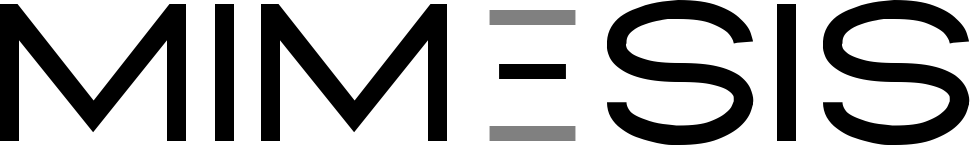
\includegraphics[width=0.2\textwidth]{mimesis.png}
\end{tcolorbox}
}


% Insert here the info that will be displayed into your Title page
% -> title of your work
\renewcommand{\title}{Title}

% -> author name and surname
\renewcommand{\author}{Ilaria Bonfanti}
% -> MSc course
\newcommand\norm[1]{\lVert#1\rVert}
\newcommand{\course}{course name}
% -> advisor name and surname
\newcommand{\advisor}{prof}
% IF AND ONLY IF you need to modify the co-supervisors you also have to modify the file Configuration_files/title_page.tex (ONLY where it is marked)
%\newcommand{\firstcoadvisor}{Name Surname} % insert if any otherwise comment
%\newcommand{\secondcoadvisor}{Name Surname} % insert if any otherwise comment
% -> academic year
\newcommand{\YEAR}{2021-2022}

%-------------------------------------------------------------------------
%	BEGIN OF YOUR DOCUMENT
%-------------------------------------------------------------------------
\begin{document}

%-----------------------------------------------------------------------------
% TITLE PAGE
%-----------------------------------------------------------------------------
% Do not change Configuration_files/TitlePage.tex (Modify it IF AND ONLY IF you need to add or delete the Co-advisors)
% This file creates the Title Page of the document
% DO NOT REMOVE SPACES BETWEEN LINES!

%\twocolumn[{\begin{@twocolumnfalse}

\AddToShipoutPicture*{\BackgroundPic}

\hspace{-0.6cm}
\includegraphics[width=0.6\textwidth]{logo_polimi_ing_indinf.eps}

\vspace{-1mm}
\fontsize{0.3cm}{0.5cm}\selectfont \bfseries \textsc{\color{bluePoli} Report}\\

\vspace{-0.2cm}
\Large{\textbf{\color{bluePoli}{\title}}}\\

\vspace{-0.2cm}
\fontsize{0.3cm}{0.5cm}\selectfont \bfseries \textsc{\color{bluePoli} \course}\\

\vspace{-0.2cm}
\fontsize{0.3cm}{0.5cm} \selectfont \bfseries Authors: \textsc{\textbf{\author}}\\

%\vspace{-0.4cm}
%\fontsize{0.3cm}{0.5cm}\selectfont \bfseries Advisor: \textsc{\textbf{\advisor}}\\

% if only ONE co-advisor is present:
%\vspace{-0.4cm}
%\fontsize{0.3cm}{0.5cm}\selectfont \bfseries Co-advisor: \textsc{\textbf{\firstcoadvisor}}\\
% if more than one co-advisors are present:
%\vspace{-0.4cm}
%\fontsize{0.3cm}{0.5cm}\selectfont \bfseries Co-advisors: \textsc{\textbf{\firstcoadvisor}}\textsc{\textbf{\secondcoadvisor}}\\

\vspace{-0.4cm}
\fontsize{0.3cm}{0.5cm}\selectfont \bfseries Academic year: \textsc{\textbf{\YEAR}}

\small \normalfont

\vspace{11pt}

\centerline{\rule{1.0\textwidth}{0.4pt}}

%\vspace{15pt}
%\end{@twocolumnfalse}}]

\thispagestyle{plain} % In order to not show the header in the first page


%%%%%%%%%%%%%%%%%%%%%%%%%%%%%%
%%     THESIS MAIN TEXT     %%
%%%%%%%%%%%%%%%%%%%%%%%%%%%%%%
Little preview
%-----------------------------------------------------------------------------
% INTRODUCTION
%-----------------------------------------------------------------------------

% \section{Introduction}

Numerical simulations play a critical role in a wide array of scientific and engineering applications, providing insights into the behavior of physical systems under various conditions. Among the most prominent techniques for performing such simulations is Finite Element Modeling (FEM). FEM discretizes a continuous domain into a mesh of finite elements, allowing for the approximation of solutions to complex partial differential equations (PDEs). However, one significant drawback of FEM is its computational intensity, especially when high resolution is required for accurate results. This research aims to explore the potential of Deep Learning (DL) techniques to accelerate FEM simulations, focusing specifically on the deformation of objects subjected to external forces.

The deformation of an object under an applied force is directly tied to the object's discretization. In FEM, the object is represented by a mesh, where the resolution of the mesh—i.e., the size and number of elements—clearly impacts the accuracy and computational cost of the simulation. High-resolution meshes can capture fine details of deformation, leading to more accurate simulations, but they are computationally expensive and time-consuming. 

The main goal of this work is to study the efficacy of a method that combines both Finite Element Modeling (FEM) and DL to obtain a realistic simulation of an object in a fraction of the time that would be required by a traditional FEM simulation. The idea is to, somehow, train a DL model to have inside the information given by the refined discretization and pass them on a coarser discretization.

The idea of using DL techniques to solve scientific problem is not new. Thanks to the rise of new frameworks and libraries, such as TensorFlow and PyTorch, it is now possible to train very complex models on large datasets in a reasonable amount of time. For the problem at hand, a lot of different approaches can be found in the existing literature: a lot of them are based on the idea that the deep learning model should predict the whole dynamic of the system, for example MeshGraphNet \cite{pfaffLearningMeshBasedSimulation2021a} or its multiscale version \cite{fortunatoMultiScaleMeshGraphNets2022}, but these are just two examples of the many possible approaches \cite{jiangMeshfreeFlowNetPhysicsConstrainedDeep2020}, \cite{djeumouNeuralNetworksPhysicsInformed2022}, \cite{hanPredictingPhysicsMeshreduced2022a}. Other methods rely on solving a time independent problem, using various architectures, such as PINNs \cite{djeumouNeuralNetworksPhysicsInformed2022} or GNNs \cite{gaoPhysicsinformedGraphNeural2022}. The proposed method falls into the second category, as it will be explained in the following sections.

One interesting solution is given by \cite{Wang_Du_Coros_Thomaszewski_2024}, where the authors extend the concept of linear modes and modal dynamics \cite{Pentland_Williams_1989} to be able to handle larger deformations. The key idea is to obtain a linear approximation of the deformation, then train a network to minimize the energy of the system, so that for every modal coordinate, the network will learn a non-linear correction, effectively learning a series of non-linear modes. This allows for faster simulations by exploiting subspace dynamics, where the simulation is performed in a reduced space to ease computational costs. The authors show that 


% \section{Smoluchowski equation}
The Smoluchowski coagulation equation models various kinds of phenomena as, for example: the evolution of a system of solid or liquid particles suspended in a gas (in
aerosol science), polymerization (in chemistry), aggregation of colloidal particles (in physics), formation of stars and planets (in astrophysics), red blood cell aggregation (in
hematology), behavior of fuel mixtures in engines (in engineering). By convention, only binary reaction will be considered.
This phenomenon is called coalescence and can be written formally as 
\[
    P_i + P_j \rightarrow P_{i+j}
\]
Under the assumption that the aggregation of cluster is the result of only Brownian motion or diffusion, the equations can be written as:
\begin{equation}
    \pdev{u_i}{t}(t,x) - d_i \Delta_x u_i(t,x) = Q_i(u) \quad \text{in } [0,T] \times \Omega,
    \label{eq:smoluchowski}
\end{equation}
where \(u_i\) is the concentration of the cluster of length \(i\), \(d_i\) is the diffusion coefficient, \(\Omega\) is the domain of the system and \(Q_i(u)\) is the gain term minus the loss term which  are defined in this way:
\begin{equation*}
    \begin{aligned}
    &Q_{g, i}=\frac{1}{2} \sum_{j=1}^{i-1} a_{i-j, j} u_{i-j} u_{j} \\
    &Q_{l, i}=u_{i} \sum_{j=1}^{\infty} a_{i, j} u_{j}
    \end{aligned}
\end{equation*}
$Q_{g,i}$ describes the increasing of concentrations of the cluster of length $i$,
$Q_{l,i}$ describes the depletion of the polymers of size $i$.
An important role is played by the coagulation coefficients $a_{i-i,j}$ which describe a situation where a polymer $i-j$ coagulates with a polymer of length $i$ to form one of length $j$, they are symmetric, indeed $a_{i,j}=a_{j,i}$.\\
The \eqref{eq:smoluchowski} is nonlinear and of infinite dimension: the existence and uniqueness of the solution is not guaranteed by the theory of RDEs. The existence of the solution as a matter of facts depends on the choice of the coagulation coefficients, of which an explicit expression is given in \cite{Bertsch}.
If there are no sources the total mass of the clusters will be conserved, but actually this is not true. In fact a particular choice of the coefficients produces a non-conservation of the total mass due to the appearance of an infinite cluster called gel, which is born from the growth of longer and longer clusters (this is known as gelation phenomenon), but will not be discussed here.
 \section{The mathematical model for Alzheimer Disease}
As mentioned above, inside the brain there exists a protein called \(\beta\) amyloid peptide ($\mathrm{A} \beta$). Healthy brains produce this protein in monomeric form, but when the mechanism breaks down \(\beta\) starts to auto agglomerate and to form senile plaques. The toxic polymers are the intermediate oligomeric formulation which causes the death of neurons. However, the causes of the AD are not yet completely known, researchers try to study this phenomenon, but the problem is that these intermediate polymers decay very soon in other longer ones. From experiments, it's not easy to study the process of coagulation, therefore the mathematical model helps us to study this process. An assumption that will be made is that 'large' assemblies do not aggregate with each other.
\subsection{Model for the brain}
\begin{figure}[H]
  \centering
  \scalebox{.5}{\incfig{domain_empty}}
  \caption{The domain $\Omega$ representing the cerebral tissue.}
  \label{fig:domain}
\end{figure}
The portion of cerebral tissue considered  in the following is represented by a bounded smooth region $\Omega_{0}\subset \mathbb{R}^3$, whereas the neurons are represented by a family of regular region $\Omega_{j}$ such that:
\begin{enumerate}[label=(\roman*)]
    \item $\bar\Omega_{j}\subset \Omega_{0}$  if   $j=1,2,\dots,\bar{M}$,
    \item $\bar\Omega_{i}\cap \bar\Omega_{j}= \emptyset$  if $i\neq j$.
\end{enumerate}
Let 
$$
\Omega := \Omega_{0} \setminus
\bigcup_{j=1}^{\bar M} \bar\Omega_{j},
$$

\noindent and consider the vector-valued function $u=(u_1,\dots, u_M)$, where $u_j=u_j(t,x)$ $(t\geq 0, t\in \mathbb{R}$ and $x\in \Omega)$ is the molar concentration at the point $x$ and at the time $t$ of a \(\beta\) assembly of $j$ monomers, while $u_M$ takes into account the aggregation of more than $M-1$ monomers. With the definition of $u_M$ it is assumed that `large' assemblies do not aggregate to each other.
Here's a brief presentation of the model made for this problem. Three different stages of the aggregation of \(\beta\) will be considered: its concentration can be modeled with $u_{i}$ with $1\leq i \leq m < M$.
The $u_{1}$ describes the concentration of monomers with the following RDE: 
$$
\frac{\partial u_{1}}{\partial t}(t, x)-d_{1} \Delta_{x} u_{1}(t, x)+u_{1}(t, x) \sum_{j=1}^{M} a_{1, j} u_{j}(t, x)=0.
$$
There is no gain term on the right-hand side because it's impossible for two monomers to coagulate and form another monomer. The loss term is given by the sum of all the possible coagulation of the monomers. 
To solve this equation boundary conditions and initial conditions are necessary.
On the external boundary homogeneous Neumann conditions are assumed, which is meant to artificially isolate the portion of tissue considered from the surrounding environment:
$$
\frac{\partial u_1}{\partial v} \equiv \nabla_{x} u_1\cdot n=0 \quad \text { on }[0, T] \times \partial \Omega.$$
In this way the flux on external fixed boundary is equal to zero, essentially isolating the portion of cerebral tissue from the rest of the world.
Boundary conditions are also needed on the boundaries of the neurons $\partial\Omega_{j}$:
$$ 
\frac{\partial u_{1}}{\partial v} \equiv \nabla_{x} u_1 \cdot n= \psi_{j} \quad \text { on } \partial\Omega_{j}.
$$
This physically models the fact that the neurons produce \(\beta\) in monomeric form. The function $\psi$ is a smooth function and it represents the quantity of \(\beta\) which is produced by the membrane of the neuron, it is a given of the problem.\\
The model considers a portion of the cerebral tissue with a bounded open set $\Omega$ in $\mathbb{R}^{3}$ with a smooth boundary $\partial \Omega$ as seen in Figure \ref{fig:domain}. The neurons in the model will be represented as holes in this domain which are distributed periodically and which have characteristic dimension $0<\epsilon<1$. The set of the domain with the holes is called the perforated domain.
It is assumed that the membrane of the neurons (holes) produces $\mathrm{A} \beta$ and that at time $t=0$ there is no production of  $\mathrm{A} \beta$ from the holes.
Let $Y$ be the unit periodicity cell $\left[0,1\left[{ }^{3}\right.\right.$ having the paving property, shown in Figure \ref{fig:unit_cell}. 
Also, denote by $T$ an open subset of $Y$ with a smooth boundary $\Gamma$, such that $\overline{T} \subset \operatorname{Int} Y$, this means that $T$ can not intersect the boundary of the set $Y$, which is the boundary of the cell. Now call with $Y^{*}=Y \backslash T$ the material part, the "solid part" of the brain. 
\begin{figure}[H]
    \centering
    \scalebox{.5}{\incfig{cell}}
    \caption{The unit periodicity cell $Y$ with the set $T$ of the interior of the hole, bounded by \(\Gamma\)}
    \label{fig:unit_cell}
  \end{figure}

Starting from this it is possible to create a perforated domain: perforate $\Omega$ by removing from it a set $T_{\epsilon}$ of periodically distributed holes defined as before. The set $T$ represents a generic neuron, and $Y^{*}$ the supporting cerebral tissue. Then define $\tau(\epsilon \overline{T})$ to be the set of all translated images $\epsilon \overline{T}$ of the form $\epsilon(k+\overline{T}), k \in \mathbb{Z}^{3}$. Then,

\[ T_{\epsilon} \coloneqq \Omega \cap \tau(\epsilon \overline{T}) . \] is the set of all the holes in the domain.

Introduce now the periodically perforated domain $\Omega_{\epsilon}$ defined by

$$
\Omega_{\epsilon} \coloneqq \Omega \backslash \bar{T}_{\epsilon},
$$
which represent all the set outside the holes. The domain $\Omega_{\epsilon}$ is shown in Figure \ref{fig:perforated_domain}.
\begin{figure}[H]
    \centering
    \scalebox{.5}{\incfig{drawing}}
    \caption{The perforated domain $\Omega_\epsilon$ representing the cerebral tissue. The neurons are represented by the holes.}
    \label{fig:perforated_domain}
  \end{figure}

Ensure that there exists a ``security zone'' where the neurons cannot touch the boundary of \(\Omega\), this is necessary to extend all the functions which live in the solid part also in the holes.
\begin{equation}
  \exists \delta>0 \text { such that dist }\left(\partial\Omega, T_{\epsilon}\right)\geq\delta.
\label{eq:security_zone}
\end{equation}
Therefore can be assumed that $\Omega_{\epsilon}$ is connected. In this scenario there are two boundaries, an internal one $\Gamma_{\epsilon}$, defined by:
$$
\Gamma_{\epsilon} \coloneqq \bigcup\left\{\partial(\epsilon(k+\bar{T})) \mid \epsilon(k+\bar{T}) \subset \Omega\right\}
$$
and an external one that is the fixed exterior boundary denoted by $\partial \Omega$:
$$
\partial\Omega_{\epsilon}\coloneqq\partial\Omega+\Gamma_{\epsilon}.
$$
It is also known that:
\begin{equation}
  \lim _{\epsilon \rightarrow 0} \epsilon\left|\Gamma_{\epsilon}\right|_{N-1}=|\Gamma|_{N-1} \frac{|\Omega|_{N}}{|Y|_{N}}
\label{eq:limit_gamma_eps}
\end{equation}
where $|\cdot|_{N}$ is the $N$-dimensional Hausdorff measure.

The aim is to pass from the microscopic scale to the macroscopic, that is, looking at the brain from 'very high' and we obtain it by performing $\epsilon \rightarrow 0$ which is the scale where clinical data exists. This process is called homogenization theory, and it is a mathematical technique that gives us some mathematical tools to perform this sort of average.
\subsection{The equations}
The system that describes the evolution of monomers is the following:
\begin{equation}
    \begin{dcases}
    \frac{\partial u_{1}^{\epsilon}}{\partial t}(t, x)-d_{1} \Delta_{x} u_{1}^{\epsilon}(t, x)+u_{1}^{\epsilon}(t, x) \sum_{j=1}^{M} a_{1, j} u_{j}^{\epsilon}(t, x)=0, & \text { in }[0, T] \times \Omega_{\epsilon},\\
    \frac{\partial u^{\epsilon}_1}{\partial v} \equiv \nabla_{x} u^{\epsilon}_1\cdot n=0, & \text { on }[0, T]\times\partial\Omega,\\
    \frac{\partial u^{\epsilon}_{1}}{\partial v} \equiv \nabla_{x} u^{\epsilon}_1 \cdot n=\epsilon \psi\left(t, x,\frac{x}{\epsilon}\right), & \text { on }[0, T] \times \Gamma_{\epsilon},\\
    u_{1}^{\epsilon}(0, x)=U_{1}, & \text{ in }\Omega_{\epsilon}.
    \end{dcases}
\label{eq:u_1_eqs}\end{equation}
Note that the $\epsilon$ is put in front of $\psi$ to prevent the divergence of the integral in a further passage, in order to avoid singularities. 
The variable $x$ is called the slow variable and the dependence between $\psi$ and $x$ models the evolution of the disease at a macroscopic scale. The variable
$\frac{x}{\epsilon}$ is called the fast scale variable, which represents the microscopic scale because the main variation of our function are on the scale of the neurons, it's in this small scale that we have a very big change.\\
From our assumptions we suppose that for $t>0$ the brain becomes sick. For technically reasons we have to assume some regularity on $\psi$ and $U_1$:
\begin{enumerate}
    \item $\psi\left(t, x, \frac{x}{\epsilon}\right) \in C^{1}(0, T ; B)$ with $B=C^{1}\left[\bar{\Omega} ; C_{\text {\# }}^{1}(Y)\right]$, where $C_{\#}^{1}(Y)$ is the subset of $C^{1}\left(\mathbb{R}^{N}\right)$ of $Y$-periodic functions;
    \item $\psi\left(t=0, x, \frac{x}{\epsilon}\right)=0$
    \item 
$U_{1}$ is a positive constant such that
\begin{equation}
  U_{1} \leq\|\psi\|_{L^{\infty}(0, T ; B)} .
\label{eq:U_1_norm}\end{equation}
\end{enumerate}
Behind these properties $\psi $ is a generic given function that should be specified in some way if one wants to make the model applicable. We will give an explicit example of it in the last part of the paper.\\
Now we will describe the evolution of oligomers: $1<m<M$. The unknown here is the concentration of a oligomer of generic length $m$
\begin{equation}
    \begin{dcases}
        \frac{\partial u_{m}^{\epsilon}}{\partial t}(t, x)-d_{m} \Delta_{x} u_{m}^{\epsilon}(t, x)+u_{m}^{\epsilon}(t, x) \sum_{j=1}^{M} a_{m, j} u_{j}^{\epsilon}(t, x)= \frac{1}{2} \sum_{j=1}^{m-1} a_{j, m-j} u_{j}^{\epsilon} u_{m-j}^{\epsilon}, & \text { in }[0, T] \times \Omega_{\epsilon},\\
        \frac{\partial u_{m}^{\epsilon}}{\partial v} \equiv \nabla_{x} u_{m}^{\epsilon} \cdot n=0,  & \text { on }[0, T]\times\partial\Omega, \\
        \frac{\partial u_{m}^{\epsilon}}{\partial v} \equiv \nabla_{x} u_{m}^{\epsilon} \cdot n=0, & \text { on }[0, T]\times\Gamma_{\epsilon}.\\ 
     u_{m}^{\epsilon}(0, x)=0 & \text{ in } \Omega_{\epsilon}
    \end{dcases}
\label{eq:u_m_eqs}\end{equation}
In this case we assume homogeneous boundary conditions also on $\Gamma_{\epsilon}$ because we assume that the neurons can't produce \(\beta\) in oligomeric form.
For what it concerns $u_{M}$, it describes the sum of all the densities of all large assemblies of \(\beta\). We are able to do that because in reality when we have a large polymer of \(\beta\) it doesn't  coagulate anymore. 
\begin{equation}
    \begin{dcases}
        \frac{\partial u_{M}^{\epsilon}}{\partial t}(t, x)-d_{M} \Delta_{x} u_{M}^{\epsilon}(t, x)= \frac{1}{2} \sum_{\mathclap{\substack{j+k\geq M\\k,j<M}}} a_{j, k} u_{j}^{\epsilon} u_{k}^{\epsilon}, & \text { in }[0, T] \times \Omega_{\epsilon},\\
        \frac{\partial u_{M}^{\epsilon}}{\partial v} \equiv \nabla_{x} u_{M}^{\epsilon} \cdot n=0,  & \text { on }[0, T]\times\partial\Omega,
        \\
        \frac{\partial u_{M}^{\epsilon}}{\partial v} \equiv \nabla_{x} u_{M}^{\epsilon} \cdot n=0, & \text { on }[0, T]\times\Gamma_{\epsilon},\\ 
        u_{M}^{\epsilon}(0, x)=0, & \text{ in }\Omega_{\epsilon}.
    \end{dcases}
    \label{eq:u_M_eqs}
\end{equation}
In this last system there isn't the loss term because we are assuming that large assemblies do not coagulate with each other.
At this point we want to go from macroscopic to microscopic, trying to compute a sort of average process. Indeed, our aim is to perform the homogenization on the set \eqref{eq:u_1_eqs}-\eqref{eq:u_m_eqs} of equations as $\epsilon \rightarrow 0$, however there is not a clear notion of convergence for the sequence $u_j^{\epsilon}$ $1\geq j \geq M$ which is defined on a varying set $\Omega_{\epsilon}$, which also is random perforated.

\begin{theorem} 
    If $\epsilon>0$, the system \eqref{eq:u_1_eqs}-\eqref{eq:u_m_eqs} has a unique solution
    $$
    \left(u_{1}^{\epsilon}, \ldots, u_{M}^{\epsilon}\right) \in C^{1+\alpha / 2,2+\alpha}\left([0, T] \times \Omega_{\epsilon}\right) \quad(\alpha \in(0,1))
    $$
    such that
    $$
    u_{j}^{\epsilon}(t, x)>0 \text { for }(t, x) \in(0, T) \times \Omega_{\epsilon}, j=1, \ldots, M .
    $$
    \label{thm:3.1}
\end{theorem}


%-----------------------------------------------------------------------------
% CONCLUSION
%-----------------------------------------------------------------------------


%---------------------------------------------------------------------------
%  BIBLIOGRAPHY
%---------------------------------------------------------------------------
%\newpage
% Remember to insert here only the essential bibliography of your work
\bibliography{bibliography.bib} % automatically inserted and ordered with this command

\end{document}
